\documentclass[xcolor=svgnames]{beamer}
\usepackage[utf8]{inputenc}
\usepackage[english]{babel}
\usepackage{numprint}
\usepackage{booktabs}
\usepackage{bibentry}
\nobibliography*
\usetheme{Proso}
\usepackage{tabularx}

\def\bysame{\leavevmode\hbox to3em{\hrulefill}\thinspace}

\title{Computerized Adaptive Practice of Factual Knowledge}
\author{Jan Papou\v{s}ek}
\institute{Masaryk University Brno}
\date{\today}

\begin{document}
% --------------------------- SLIDE --------------------------------------------
\frame[plain]{\titlepage}
% ------------------------------------------------------------------------------
% --------------------------- SLIDE --------------------------------------------
\begin{frame}
	\begin{itemize}
		\item efficient way of memorizing facts
		\item no or minimal assistance of teacher
		\item at the same time:
			\begin{itemize}
				\item estimating learners' knowledge
				\item their learning
			\end{itemize}
		\item online (available to large number of learners)
	\end{itemize}
\end{frame}
% ------------------------------------------------------------------------------
% --------------------------- SLIDE --------------------------------------------
\begin{frame}
	\frametitle{Outline}
	\begin{itemize}
		\item models estimating learners' performance and knowledge
		\item practice control (instructional policy)
		\item evaluation
	\end{itemize}
\end{frame}
% ------------------------------------------------------------------------------
% --------------------------- SLIDE --------------------------------------------
\begin{frame}
	\frametitle{Models}
	\begin{itemize}
		\item items are independent to each other
		\item forgetting
		\item repetition and spacing effect
		\item varied prior knowledge
		\item often relative difficulty of items is the same for all learners
	\end{itemize}
\end{frame}
% ------------------------------------------------------------------------------
% --------------------------- SLIDE --------------------------------------------
\begin{frame}
	\frametitle{Models: forgetting and spacing effect}
	\begin{center}
		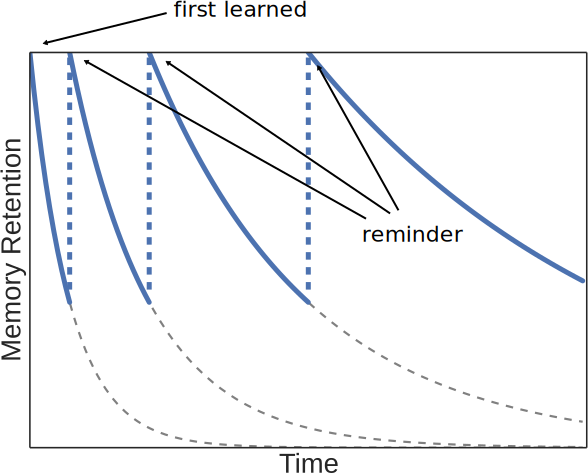
\includegraphics[width=0.7\textwidth]{figure/forgetting_curves.pdf}
	\end{center}
\end{frame}
% ------------------------------------------------------------------------------
% --------------------------- SLIDE --------------------------------------------
\begin{frame}
	\frametitle{Models: overview}
	(data) community focuses on procedural knowledge (math, programming)
	\begin{itemize}
		\item Bayesian Knowledge Tracing and its extensions
	\end{itemize}

	\bigskip
	estimation of prior knowledge can be inspired by IRT
	\begin{itemize}
		\item Rasch, Elo rating system (chess)
	\end{itemize}

	\bigskip
	learning of factual knowledge:
	\begin{itemize}
		\item PFA (too simple)
		\item ACT-R (not tested online with larger dataset)
	\end{itemize}
\end{frame}
% ------------------------------------------------------------------------------
% --------------------------- SLIDE --------------------------------------------
\begin{frame}
	\frametitle{Practice Control}
	\begin{itemize}
		\item inner vs. outer loop
		\item sequencing
			\begin{itemize}
				\item balance between over-practice and under-practice
				\item zone of proximal development
			\end{itemize}
		\item questions
			\begin{itemize}
				\item number of options
				\item competitiveness of options
			\end{itemize}
	\end{itemize}
\end{frame}
% ------------------------------------------------------------------------------
% --------------------------- SLIDE --------------------------------------------
\begin{frame}
	\frametitle{Practice Control: sequencing}
	\begin{columns}[2]
		\column{.5\textwidth}
			\begin{center}
				\includegraphics[width=0.9\textwidth]{figure/practice_progress_a}
			\end{center}
		\column{.5\textwidth}
			\begin{center}
				
\includegraphics[width=0.9\textwidth]{figure/practice_progress_b}
			\end{center}
	\end{columns}
\end{frame}
% ------------------------------------------------------------------------------
% --------------------------- SLIDE --------------------------------------------
\begin{frame}
	\frametitle{Practice Control: options}
	\begin{center}
		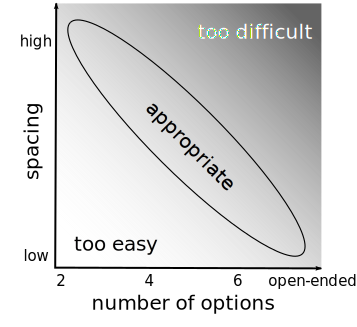
\includegraphics[width=0.7\textwidth]{figure/options_vs_spacing}
	\end{center}
\end{frame}
% ------------------------------------------------------------------------------
% --------------------------- SLIDE --------------------------------------------
\begin{frame}
	\frametitle{Evaluation}
	learning and learners' willingness to use the system
	\begin{itemize}
		\item new data (A/B experiments, multi-armed bandits, \ldots)
		\item historical data (performance of predicitve models, \ldots)
		\item synthetic data
	\end{itemize}
\end{frame}
% ------------------------------------------------------------------------------
% --------------------------- SLIDE --------------------------------------------
\begin{frame}
	\frametitle{Aims of the Thesis}
	\begin{itemize}
		\item model estimating leaners' knowledge
			\begin{itemize}
				\item prior knowledge
				\item forgetting
				\item spacing effect
			\end{itemize}
		\item strategies for practice control
			\begin{itemize}
				\item appropriate difficulty
			\end{itemize}
		\item evaluation
			\begin{itemize}
				\item online experiments: learning, motivation
				\item synthetic data: model vs. practice control
			\end{itemize}
	\end{itemize}
\end{frame}
% ------------------------------------------------------------------------------
% --------------------------- SLIDE --------------------------------------------
\begin{frame}
	\frametitle{Achieved Results: slepemapy.cz}
	\begin{center}
		\includegraphics[width=0.9\textwidth]{figure/slepemapy_spain_highlighted.png}
	\end{center}
\end{frame}
% ------------------------------------------------------------------------------
% --------------------------- SLIDE --------------------------------------------
\begin{frame}
	\frametitle{Achieved Results: slepemapy.cz}
	\begin{itemize}
		\item $\geq$ \numprint{14000000} answers in total
		\item per month:
			\begin{itemize}
				\item \numprint{1000000} answers
				\item \numprint{10000} users
			\end{itemize}
	\end{itemize}

	\medskip
	\begin{itemize}
		\item source of data
		\item platform for online experiments
	\end{itemize}
\end{frame}
% ------------------------------------------------------------------------------
% --------------------------- SLIDE --------------------------------------------
\begin{frame}
	\frametitle{Achieved Results: publications}
	\begin{itemize}
		\item \bibentry{papousek2015impact}
		\begin{itemize}
			\item best student paper award
		\end{itemize}
		\item \bibentry{papousek2015analysis}
		\item \bibentry{papousek2014adaptive}
	\end{itemize}
\end{frame}
% ------------------------------------------------------------------------------
% --------------------------- SLIDE --------------------------------------------
\begin{frame}
	\frametitle{Achieved Results: publications}
	\begin{itemize}
		\item \bibentry{niznan2015exploring}
	\end{itemize}
	\textbf{forthcoming}
	\begin{itemize}
		\item \bibentry{pelanek2016learner}
		\item \bibentry{papousek2015dataset}
	\end{itemize}
\end{frame}
% ------------------------------------------------------------------------------
% --------------------------- SLIDE --------------------------------------------
\begin{frame}
	\frametitle{Achieved Results: publications}
	\textbf{submitted}
	\begin{itemize}
		\item \bibentry{papousek2016evaluation}
		\item \bibentry{pelanek2016impact}
	\end{itemize}
	\bibliographystyle{amsplain}
	\nobibliography{proposal}
\end{frame}
% ------------------------------------------------------------------------------
% --------------------------- SLIDE --------------------------------------------
\begin{frame}
\frametitle{Proposed Plan of Work}
\begin{tabularx}{\textwidth}{rX}
	\textbf{Autumn 2015} &
		\vspace{-0.5cm}
		\begin{enumerate}
			\item Design and implementation of methodology for evaluation of the impact
				of adaptive practice on a user's learning.
			\item Evaluation of already existing algorithms for practice control using the
				developed methodology.
			\item Deployment of a new version of the system providing the practice of
				geography that will be able to adopt a new student model.
		\end{enumerate}
\end{tabularx}
\end{frame}
% ------------------------------------------------------------------------------
% --------------------------- SLIDE --------------------------------------------
\begin{frame}
\frametitle{Proposed Plan of Work}
\begin{tabularx}{\textwidth}{rX}
	\textbf{Spring 2016} &
		\vspace{-0.5cm}
		\begin{enumerate}
			\item Design and implementation of a new student model of learning of
				facts.
			\item Development of strategies for practice control cooperating with the
				proposed student model.
		\end{enumerate}\\
	\textbf{Autumn 2016} &
		\vspace{-0.5cm}
		\begin{enumerate}
			\item Evaluation of the proposed strategies.
			\item Experiments with synthetic data.
		\end{enumerate}\\
	\textbf{Spring 2017} &
		\vspace{-0.5cm}
		\begin{enumerate}
			\item Finishing and submitting the thesis.
		\end{enumerate}
\end{tabularx}
\end{frame}
% ------------------------------------------------------------------------------
\end{document}
